\documentclass[oneside]{book}

%%%%%%%%%%%%%%%%%%%%%%%% PREAMBLE %%%%%%%%%%%%%%%%%%%%%%%%

% Packages
\usepackage{amsmath}
\usepackage{listings}
\usepackage{graphicx}
% To get code colors
\usepackage{xcolor}
\usepackage{wrapfig}

\setlength{\parindent}{0pt}
% Change listings name to "Code"
\renewcommand{\lstlistingname}{Code}
% Define colors for codestyles
\definecolor{codegreen}{rgb}{0,0.6,0}
\definecolor{codegray}{rgb}{0.5,0.5,0.5}
\definecolor{codepurple}{rgb}{0.58,0,0.82}
\definecolor{backcolour}{rgb}{0.95,0.95,0.92}
% Solidity code syntax
% Define colors for codestyles
\definecolor{codegreen}{rgb}{0,0.6,0}
\definecolor{codegray}{rgb}{0.5,0.5,0.5}
\definecolor{codepurple}{rgb}{0.58,0,0.82}
\definecolor{backcolour}{rgb}{0.95,0.95,0.92}

\lstdefinelanguage{Solidity}{
	keywords=[1]{anonymous, assembly, assert, balance, break, call, callcode, case, catch, class, constant, continue, constructor, contract, debugger, default, delegatecall, delete, do, else, emit, event, experimental, export, external, false, finally, for, function, gas, if, implements, import, in, indexed, instanceof, interface, internal, is, length, library, log0, log1, log2, log3, log4, memory, modifier, new, payable, pragma, private, protected, public, pure, push, require, return, returns, revert, selfdestruct, send, solidity, storage, struct, suicide, super, switch, then, this, throw, transfer, true, try, typeof, using, value, view, while, with, addmod, ecrecover, keccak256, mulmod, ripemd160, sha256, sha3}, % generic keywords including crypto operations
	keywordstyle=[1]\color{magenta}\bfseries,
	keywords=[2]{address, bool, byte, bytes, bytes1, bytes2, bytes3, bytes4, bytes5, bytes6, bytes7, bytes8, bytes9, bytes10, bytes11, bytes12, bytes13, bytes14, bytes15, bytes16, bytes17, bytes18, bytes19, bytes20, bytes21, bytes22, bytes23, bytes24, bytes25, bytes26, bytes27, bytes28, bytes29, bytes30, bytes31, bytes32, enum, int, int8, int16, int24, int32, int40, int48, int56, int64, int72, int80, int88, int96, int104, int112, int120, int128, int136, int144, int152, int160, int168, int176, int184, int192, int200, int208, int216, int224, int232, int240, int248, int256, mapping, string, uint, uint8, uint16, uint24, uint32, uint40, uint48, uint56, uint64, uint72, uint80, uint88, uint96, uint104, uint112, uint120, uint128, uint136, uint144, uint152, uint160, uint168, uint176, uint184, uint192, uint200, uint208, uint216, uint224, uint232, uint240, uint248, uint256, var, void, ether, finney, szabo, wei, days, hours, minutes, seconds, weeks, years},	% types; money and time units
	keywordstyle=[2]\color{teal}\bfseries,
	keywords=[3]{block, blockhash, coinbase, difficulty, gaslimit, number, timestamp, msg, data, gas, sender, sig, value, now, tx, gasprice, origin},	% environment variables
	keywordstyle=[3]\color{violet}\bfseries,
	identifierstyle=\color{black},
	sensitive=false,
	comment=[l]{//},
	morecomment=[s]{/*}{*/},
	commentstyle=\color{codegreen}\ttfamily,
	stringstyle=\color{codepurple}\ttfamily,
	morestring=[b]',
	morestring=[b]"
}

\lstdefinestyle{solStyle}{
	language=Solidity,
	backgroundcolor=\color{backcolour},
	extendedchars=true,
	basicstyle=\footnotesize\ttfamily,
	showstringspaces=false,
	breakatwhitespace=false,
	showspaces=false,
	numbers=left,
	numberstyle=\tiny\color{codegray},
	numbersep=5pt,
	tabsize=4,
	breaklines=true,
	showtabs=false,
	captionpos=b
}

\lstdefinestyle{defaultStyle}{
    backgroundcolor=\color{backcolour},
    commentstyle=\color{codegreen},
    keywordstyle=\color{magenta},
    numberstyle=\tiny\color{codegray},
    stringstyle=\color{codepurple},
    basicstyle=\ttfamily\footnotesize,
    breakatwhitespace=false,
    breaklines=true,
    captionpos=b,
    keepspaces=true,
    numbers=left,
    numbersep=5pt,
    showspaces=false,
    showstringspaces=false,
    showtabs=false,
    tabsize=4
}

%%%%%%%%%%%%%%%%%%%%%%%% TITLE %%%%%%%%%%%%%%%%%%%%%%%%

\title{Secureum CARE-X:\\Certora Prover\\\&\\AAVE Protocol}
\date{July 11, 2022}

% Document
\begin{document}

    \maketitle

    \chapter{Auditing and Formal Verification: Better together}

    \section{Auditing}

    It's the procedure that a human reviews the code either internally or externally.
    The review aims to check the correctness of the code and the documentation.
    It's either done by a white hacker or an auditor.

    \begin{itemize}
        \item Review the documentation and the code
        \item Check against common mistakes
        \item Identify issues
        \item Evaluate the security of the process
    \end{itemize}

    It's used in many domains, but in smart contract it is mandatory.\\

    Since formal verification is less clear, let's address it from a sort of common ground.
    We all know from \texttt{unix} this very useful software called \texttt{diff} which compares two files: it basically shows you the difference between the files (which lines are the same, which lines are different\dots).
    This useful technology has been around for ages and it's used in many domains.\\

    For the purpose of this talk, you can think of formal verification as a smart way to do this \texttt{diff}.

    \begin{figure}[htbp!]
        \centering
        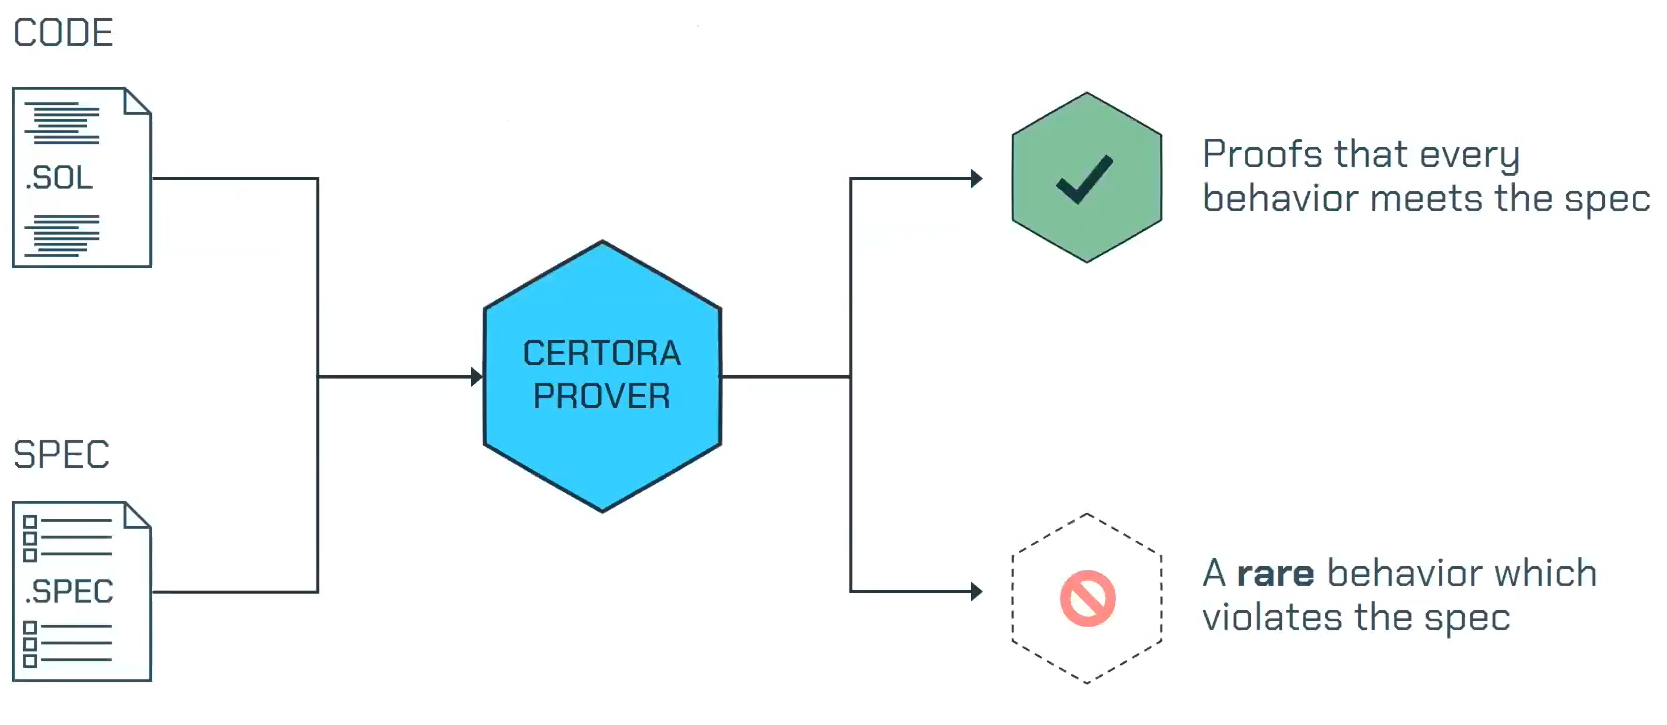
\includegraphics[width=\linewidth]{img/formal_verification_diff}
    \end{figure}

    The idea is that we compare between the code on one side and the specification on the other side.
    These are sort of two separate files: one of them is written in code, say \texttt{Solidity} or \texttt{Rust}, while the other one is written in the spec language.\\

   What this does is providing a proof that all the behaviors of the code (and there are usually many, even infinite) satisfy the rules or it can identify a behavior that could be pretty rare, which could also be found by an auditor.
    So formal verification may show you some input that violates the spec.\\

    The interesting thing is that this formal verification can actually give you bugs.
    Some people, as a joke, say that formal verification is the art of making sure that your code and the spec have the same kind of bugs.\\

    Formal verification is a mature field (like many others in computer science), but it has been through different kinds of phases (like artificial intelligence and others).\\

    Formal verification goes back to Sir Alan Turing who explained in how to do this formal verification.

    Then followed the golden years, where Robin Milner, Tony Hoare, Edgar Dijkstra, Patrick Cousot and Bob Floyd came with this technique for formal methods.\\

    All of them, with the exclusion of Patrick Cousot, they got the Turing award for that.
    These techniques they invented made programming into a science.
    The biggest quote is by Dijkstra was that this was the only way to prove that the code was correct.

    \pagebreak

    \begin{figure}[htbp!]
        \centering
        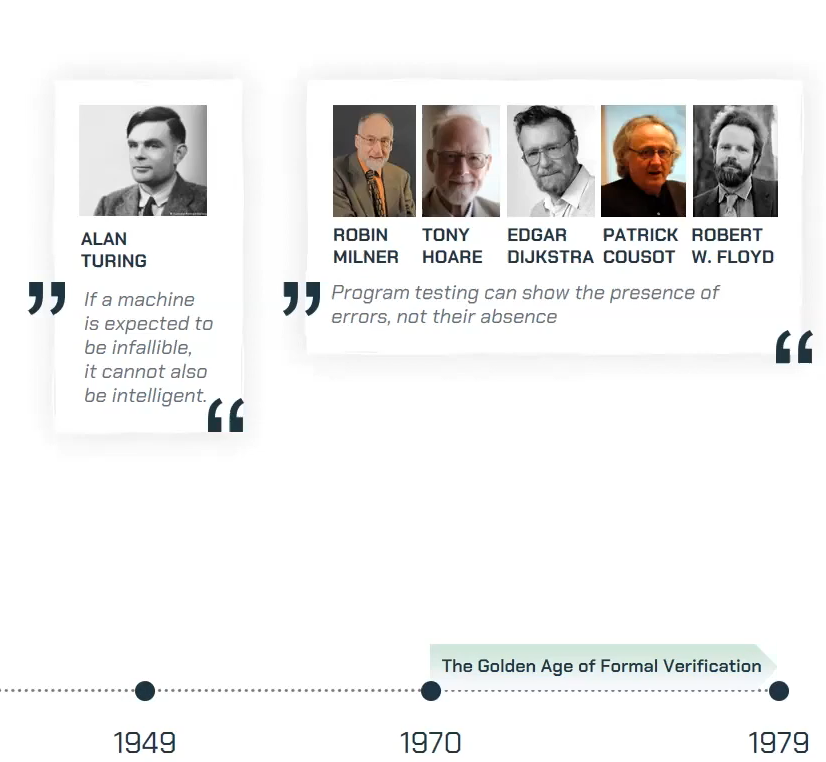
\includegraphics[width=\linewidth]{img/formal_verification_history_1}
    \end{figure}

    That was very nice but it was in fact a bit naive.
    What happened in 1979 is that a lot of people, in particular Demillo, Lipton and Perlis, came up with a paper on not using formal verification.
    They explained why this method will never work.\\

    It was very bad for the field showing that the technique of formal verification was very very hard and explaining with rational reason why formal method was not the way to go.\\

    That, however, didn't prevent people from working on formal methods.
    There was a lot of work that went towards that direction, in particular the work done by the Microsoft research team which got the device driver formal verification to work to eliminate the blue screens in Microsoft Windows.\\

    \vfill

    \begin{figure}[htbp!]
        \centering
        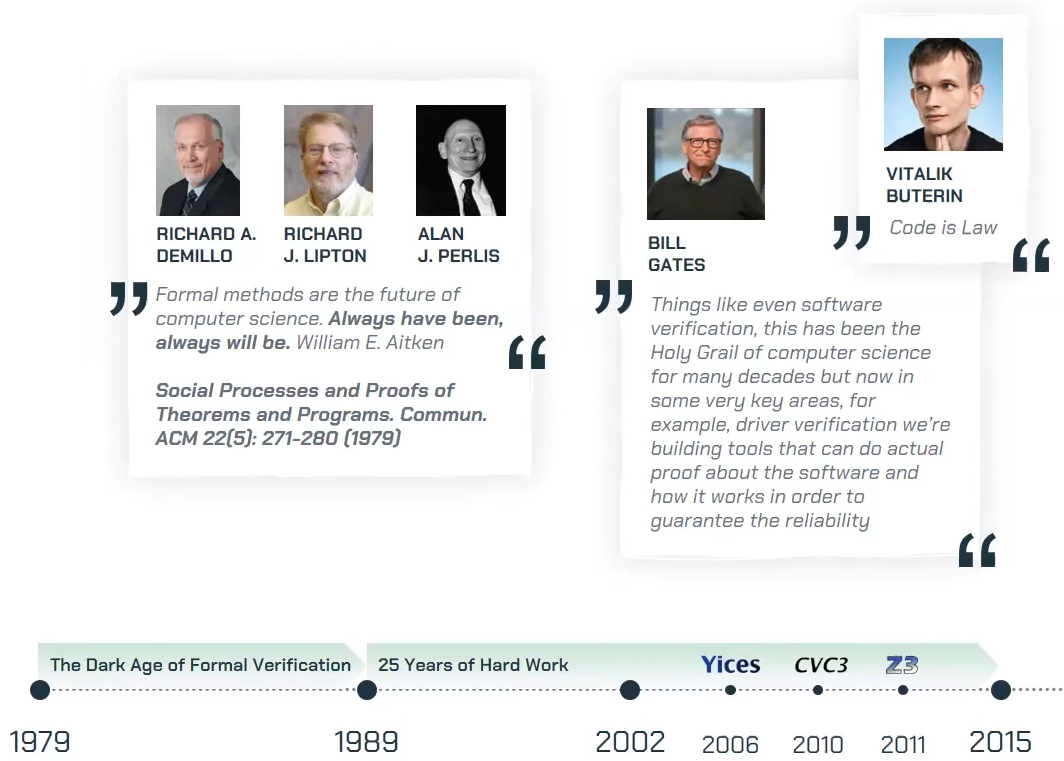
\includegraphics[width=\linewidth]{img/formal_verification_history_2}
    \end{figure}

    There are a lot of very which are used now like the \texttt{Yikes} tool (which came from the Stanford Research Institute), \texttt{CVC} (which came from the Iowa and Stanford University) and \texttt{Z3} which came from Microsoft Research.\\

    But maybe the biggest thing for us, at least taking this thing to a practical merit, is actually the idea that smart contract or ``the code is law".
    Smart contracts yield a very interesting application of formal methods because you have small code carrying a lot of value, so the scalability issue does not exist if you can get formal verification to work.
    This is a very very interesting domain.\\

    In addition, the fact that the smart contracts are immutable makes you really want to perform formal verification before the code is deployed.

    \subsection{Invariants}

    The biggest value of formal verificatiom comes already from the specification.
    You write some properties of your code and you write the desired properties of the code.
    This is called \textbf{invariant}.

    \begin{itemize}
        \item Necessary parts of code documentation
        \item\textbf{Desired} properties of the code
        \item\textbf{What} the code is supposed to do (not how)
    \end{itemize}

    This is actually already useful for auditing.
    In fact, we think that the auditor needs to review the specification.
    Here are some examples:

    \begin{itemize}
        \item No double spend
        \item Liquidation increases the amount of collateral
        \item The order of deposits does not matter (it does not matter if I deposit $x$ and then $y$, or $x+y$)
    \end{itemize}

    There are languages employed to write specifications

    \begin{itemize}
        \item TLA+ (by Leslie Lamport)
        \item Assert and require (SMTChecker)
        \item Certora Verification Language (CVL)
    \end{itemize}

    A very very simple case of invariants is the following case: imagine you have that $x+y\geq 2$.
    We are interested in finding the invariant that separates the bad state (the set of $x$ and $y$ that do not satisfy $x+y\geq 2$) from the good stuff.\\

    \textbf{There are some interesting invariants in \texttt{DeFi}}:

    \begin{itemize}
        \item For every borrowed token, there is sufficient collateral borrow
        \item The sum of balances is equal to the total amount
        \item\texttt{LiquidityShares}$>0\Leftrightarrow$\texttt{SystemHolding}$>0$
        \item Each token has a unique entry (index in array)
        \item Reward does not exceed \texttt{max value}
    \end{itemize}

    So you can come up with interesting invariants.
    This is actually the biggest part of formal verification.
    Maybe just to clarify, there are bad invariants and there are many ways to write bad invariants.
    Here are some examples:

    \begin{itemize}
        \item Too permissive\\
            $x+2>x \Rightarrow$ this is a tautology (it's always true)\\
            $2x<x \Rightarrow 5>7 \Rightarrow$ this is also a tautology (it's always false)
        \item Too restrictive
            $$x=3\vee x=4$$
    \end{itemize}

    \subsection{Reachable states // \textit{Hoare Triples}}

    So let's talk about how to write invariants.
   The idea of Hoare is that you every execution of the contract starting in a state in $P$ results in a state in $Q$, where $P,Q\subset X$, being $X$ the total space of states.\\

    Note that states belonging to $P$ and $Q$ satisfy the corresponding invariants $p$ and $q$.
    So it's a condition on your invariant: $p$ is what you are assuming and $q$ is what you are ensuring.\\

    This is how you build systems and which allow you to compose systems.
    It requires that for every execution that you start with a state which satisfies $p$, it has to finish with a state that satisfies $q$.

    \begin{lstlisting}[language=Solidity, style=SolStyle]
if P then {
    Contract;
    assert Q;
}
\end{lstlisting}

    So basically you see here that it doesn't require anything on the states outside it.
    The only situation that is forbidden is that you start with a state which is good ($P$) and you end up in a state which is bad (not $Q$).\\

    The art of formal verification is writing these rules and then using them either to find out or prove the actions.
    They are also sometimes called \textbf{safety}.
    Intuitively safety means that nothing bad will happen, as opposed to liveness (something good will happen).\\

    \pagebreak

    \section{Spec vs. Code}

    \begin{table}[htbp!]
        \centering
        \begin{tabular}{|c|c|}
            \hline
            \texttt{SPEC}&\texttt{CODE}\\
            \hline
            Declarative (what)&Imperative (how)\\
            \hline
            Not meant to be executed&Efficient\\
            \hline
            Partial&Complete\\
            \hline
            Reusable&Tailor made\\
            \hline
            Captures the essence from & Describes an efficient way to\\
            a user perspective & realize the specification\\
            \hline
            Readable and small&Well documented but can be complex\\
            \hline
            \textbf{Can have bugs}&\textbf{Can have bugs}\\
            \hline
        \end{tabular}
    \end{table}

    Annotations:

    \begin{itemize}
        \item By declarative, it is meant that the code is actually executing things.
            Although, of course, there are declarative languages, \texttt{Solidity} or \texttt{Rust} are imperative.
        \item By complete, it is meant that inside the code, it is described how everything is executed.
        \item By partial, it is meant that it just describes some common security properties.
        \item By reusable, it is meant both for different versions of the same code and different defaults.
            For example the cases of \texttt{AAVE} and \texttt{Compound}: they're implementing different things but they still satisfy similar rules.
    \end{itemize}

    Let's consider the following simple buggy program:

    \begin{lstlisting}[language=Solidity, style=SolStyle]
transfer (address from, address to, uint256 amount) {
    require (balances [from] >= amount);
    balancesFrom = balances[from] - amount;
    balancesTo = balances[to] + amount;
    balances[from] = balancesFrom;
    balances[to] = balancesTo;
}
\end{lstlisting}

    This is a transfer which is buggy and a human can find this bug usually very easily.
    In order to find this bug, you have to tell the \texttt{Certora Prover} what you are expecting from the contract.
    The simplest thing to ask for is that the total is equal to the sum of the balances, which is an \texttt{ERC20}.\\

   $$
   \text{Invariant:  \texttt{Total}}=\sum_{a:=\text{\texttt{address}}}\text{\texttt{balances[a]}}
   $$

    Then the system will automatically identify a bug, which is basically self-liquidation.\\

    The idea is that Alice transfers money to herself, yielding in an increase of her balance.

    \begin{lstlisting}[language=Solidity, style=SolStyle]
{
    from="Alice"
    to="Alice"
    amount=18
    old.balances("Alice") = 20
    new.balances("Alice") = 38
}
\end{lstlisting}

    \texttt{Certora Prover} found it automatically by comparing the call to the specification (using this invariant/rule you wrote).

    When you correct the code, then it will not tell you that this code does not have a bug, but it will still at least tell you that this bug holds, so it gives you more guarantee of the code.\\

    \begin{align*}
        &\text{\texttt{Total}}=\sum_{a:=\text{\texttt{address}}}\text{\texttt{old.balances[a]}}\\
        &\text{\texttt{Total}}=\sum_{a:=\text{\texttt{address}}}\text{\texttt{new.balances[a]}}
    \end{align*}

    It tells you that this would hold: that in fact the sum of the balance before and after remains the same.\\

    The basic thing about formal verification is that the we are looking for behaviors which are \textbf{bad}.
    So the developer specifies the \textbf{desired} behavior and the computer searches through \textbf{potentially infinite} behaviors.
    This is a very very hard problem from a computational point of view.
    It ranges from $np$ complete to undecidable, but in fact there are tools including \texttt{Certora Prover} that solve this in many many cases and in code which ranges from $50$ LOC to sometimes $5\cdot 10^3$ LOC and more.\\

    When these tools do not work, then the developer can help.
    There are different mechanism for interaction.\\

    The simplest is \textbf{modularity}: you bring the code into several pieces and you separately verify each code with respect to the specification.\\

    So basically formal verification in practice can come up with proofs, bugs or timeout (in some cases, the tool runs out of time and doesn't prove anything nor finds any bugs).
    That's, of course, useless and, although we are trying to avoid it, it's unavoidable when the code gets too complex (the problem is undecidable).\\

    This means that a human can always write a program with a property for which this tool fails.\\

    Notice that this tool is still more useful than say common static analysis, methods because it doesn't have false positives nor false negatives in a sense that every time it gives you a bug, it is in fact a bug which violates the rule, and every time it tells you that the rule holds, it really holds.\\

    In the end, it's increasing your knowledge about your code.\\

    Other things to notive about formal verification are

    \begin{itemize}
        \item It is the only method that proves properties
        \item However, it is \textbf{useless} without good specs
        \item But sometimes generic rules are sufficient
    \end{itemize}

    Of course, when you work with formal verification and especially when you are a beginner, some level of \textbf{paranoia} is useful, so if the formal verification gave you a bug, check it out of course.
    But if the formal verification does not report a bug, then the first thing to check is that whether there's a problem with your specification.\\

    You can mutate the program (in the sense that you manually insert a bug) and try to see that the formal verification finds it.
    So basically check the usefulness of the tool by changing your program and see if if the rule is valid.\\

    \pagebreak

    \section{A technical example: The \texttt{SUSHISWAP} protocol}

    \begin{wrapfigure}[5]{l}{0.25\textwidth}
        \centering
        
\includegraphics[width=0.25\textwidth]{img/sushiswap}
    \end{wrapfigure}
    ~
    \begin{itemize}
        \item Sophisticated protocol (established 2020)
        \item Decentralized exchange
        \item Tricky code \& thousands of LOC
        \item TVL \$2.17B
    \end{itemize}

    We're going to see some examples of useful invariants that are useful even beyond the \texttt{SUSHISWAP} protocol.\\

    Let's start with the simplest version of liquidation: the \texttt{KASHIPAIR}.

    \begin{figure}[htbp!]
        \centering
        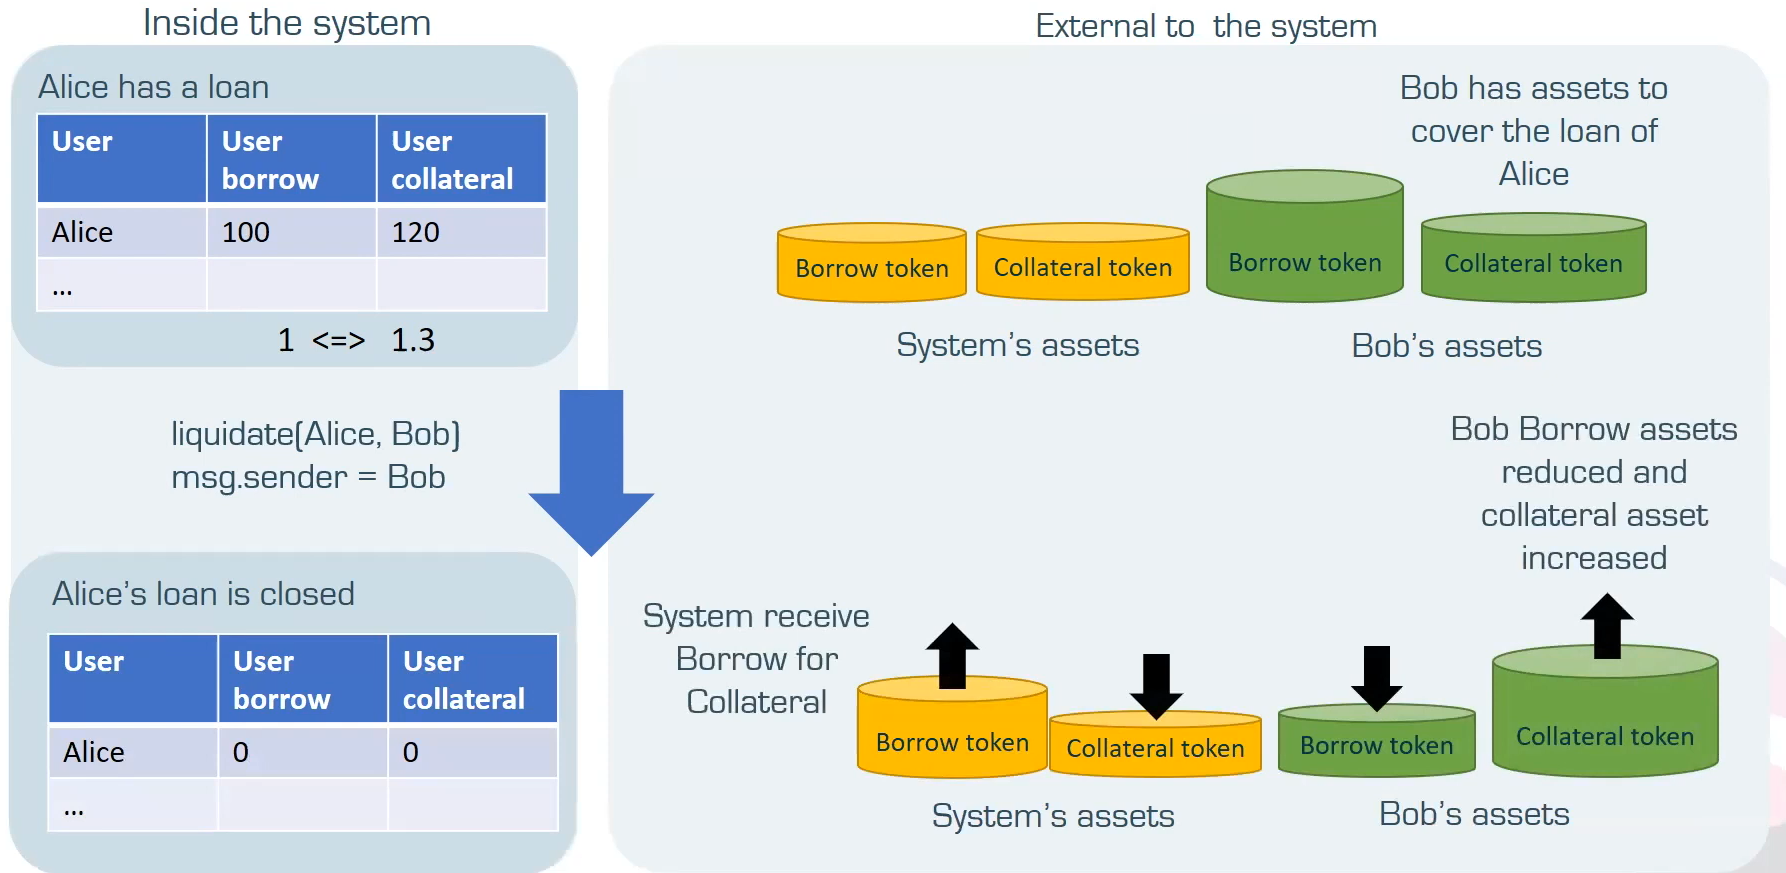
\includegraphics[width=\linewidth]{img/kashipair}
    \end{figure}

    Above you can see that there is thet the state outside of the system and the state inside of the system inside the system.\\

    Alice, inside the system, borrows 100 \texttt{Eth} and the collateral is 120.
    Suppose now that the value that the ratio is $1:1.3$, this means that at this point Alice is in trouble: her collateral does not suffice for her goal.\\

    So somebody else has the incentive to come and cover Alice's loan.
    You see here Bob has sufficient borrow and can cover Alice's loan.
    So it executes \texttt{liquidate(Alice, Bob)} with the message sender being Bob.
    What will happen is that Alice's loan is covered and Bob would get some reward because he can get the collateral and the system also covered the loan.\\

    Basically this is an idea where actually Bob has the incentive to cover Alice's loan.
    It's implemented in the \texttt{liquidate} procedure.
    Here we have a simplified version of the code:

    \begin{lstlisting}[language=Solidity, style=SolStyle]
function batchCalls(address[] callee, bytes[] calldata datas) {
    ...
    callee[i].call(datas[i]);
}

/* Liquidation of a user that is in insolvent state
    user - address to liquidate
    to - address to receive collateral */

function liquidate(address user, address to) {
    require(!_isSolvent(user));

    borrow = UserBorrowAmount[user];
    collateral = userCollateralAmount[user];

    userBorrowAmount[user] = 0;
    userCollateralAmount[user] = 0;

    borrowToken.transferFrom(msg.sender, address(this), borrow);
    collateralToken.transfer(to, collateral);
}
    \end{lstlisting}

    As you can see, there is this \texttt{batchCalls} which is calling \texttt{liquidate}.
    \texttt{batchCalls} is wrapping several transactions into one.
    Now suppose you want to check it in your audition.
    You can think of applying useful methods like unit testing.
    However, there are a lot of behaviors that you have to check: any contact list (see \texttt{callee}), any function (see \texttt{datas})\dots That's very very hard to find.\\

    When you are reviewing this code, although it is simple, it can be pretty tricky.
    
    \subsection{Good properties of liquidation}
    
    So we will want to define some rules that define good properties of liquidation and this is a good property.
    For example, in \texttt{SUSHISWAP} we have the following rule:\\


    \textbf{Collateral} token balance and \textbf{Borrow} token balance are complementary: if \textbf{Borrow} token balance increases, then \textbf{Collateral} token balance decreases.\\

    This is a property that you're looking for outside the system, independent of its implementation.
    For example, if the collateral is $100$ and the borrow is $60$, then you can increase the borrow to $70$ and reduce the collateral to $90$.\\

    So we're going to write the code so that this invariant is ensured.
    This is exactly the Hoare triple: you take this \texttt{liquidate} and you surround it by rules:

    \begin{align*}
        &\text{\texttt{\{b = BorrowT.balanceOf(System)}}\wedge\text{\texttt{c = CollateralT.balanceOf(System)\}}}\\
        &\hspace{1cm}\text{\texttt{liquidate(x, y)}}\\
        &\text{\texttt{\{BorrowT.balanceOf(System)}}>\text{\texttt{b}}\Leftrightarrow\text{\texttt{CollateralT.balanceOf(System)}}<\text{\texttt{c\}}}\\
    \end{align*}

    You can actually read in the verification report that this is the property that we are trying to verify.
    So we run the tool with said rule:

    \begin{lstlisting}[language=Solidity, style=SolStyle]
rule antimonocityOfLiquidation () {
    env e;
    address user;
    address to;

    collateralBefore = collateralToken.balanceOf(this);
    borrowBefore = borrowToken.balanceOf(this);
    ...

    liquidate(e, user, to);

    collateralAfter = collateralToken.balanceOf(this);
    borrowAfter = borrowToken.balanceOf(this);

    assert(borrowBefore < borrowAfter <=> collateralBefore > collateralAfter);
}
\end{lstlisting}

    After running \texttt{Certora Prover} with this rule, it returns a violation of the atomicity of liquidation.
    It gives you the trace and shows the EVM state of the transaction.
    It is, in fact, a very interesting and severe bug.\\

    \begin{figure}[htbp!]
        \centering
        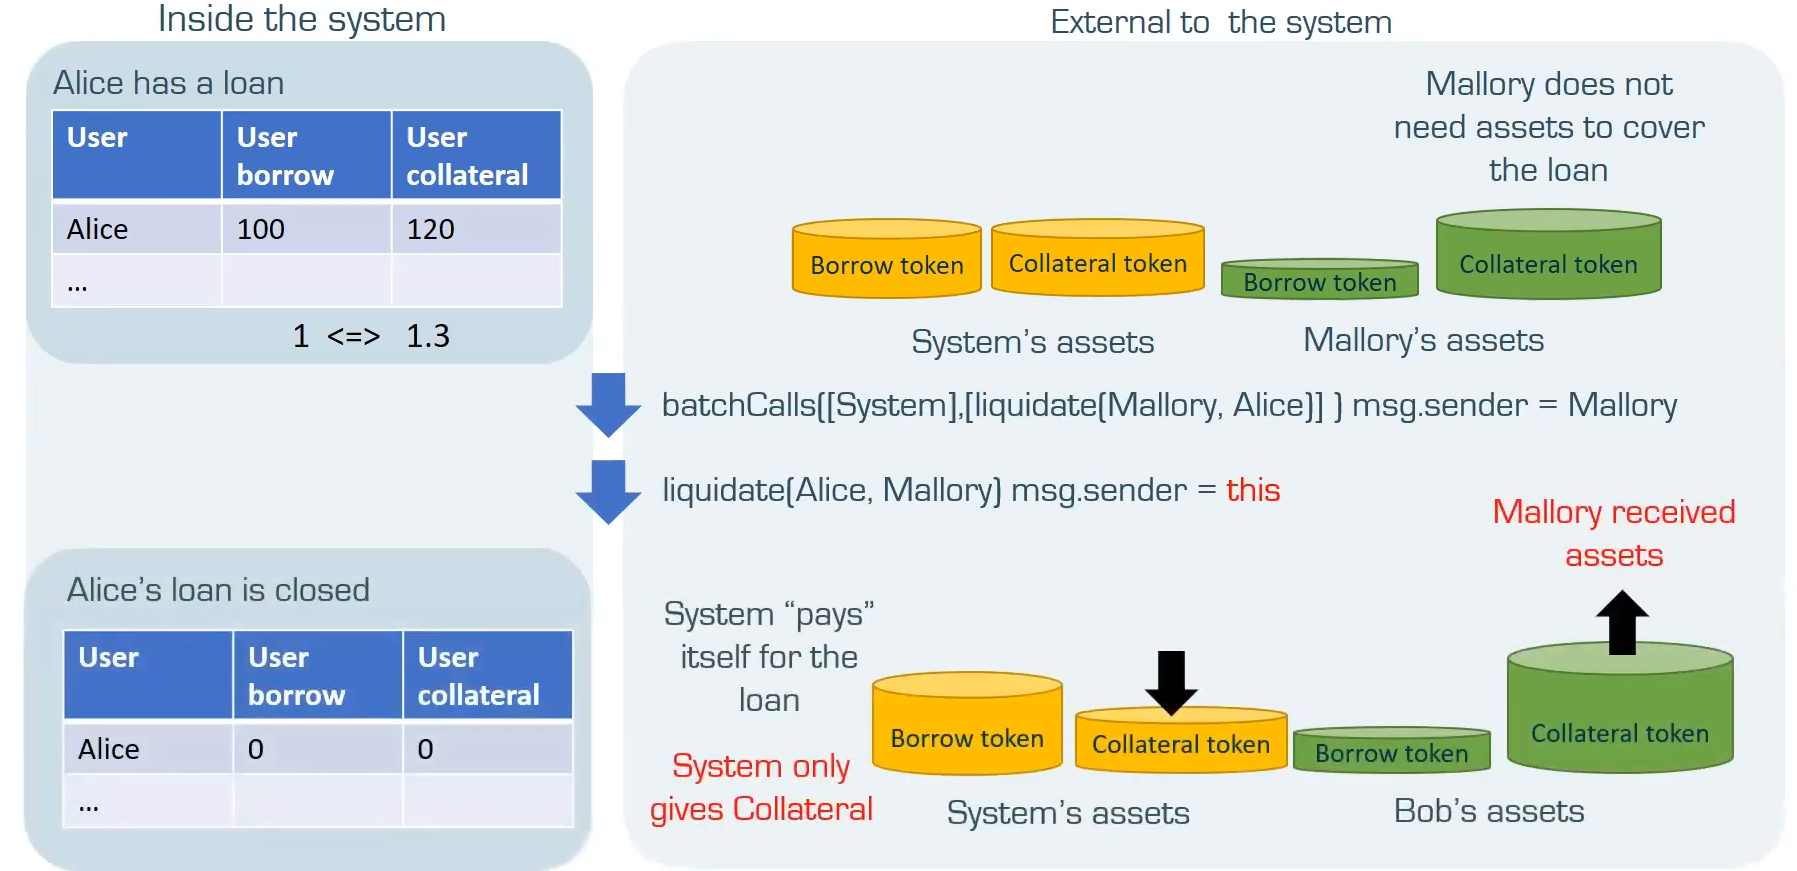
\includegraphics[width=\linewidth]{img/kashipair_bug}
    \end{figure}

    Basically, the system allowed that Mallory could gain money without actually paying anything.
    So Mallory doesn't have anything to cover and she is calling, with the message sender being herself.
    As a result, there is this liquidation and the system pays itself.
    So Alice's loan is covered, Mallory pays nothing and gets Alice's collateral.\\

    That, of course, is a very very bad behavior.
    Luckily, this was told to the Sushi team before it was deployed and they changed the code.\\

    There are different ways to change the code.
    For example adding

    \begin{lstlisting}[language=Solidity, style=SolStyle]
require(msg.sender != address(this));
\end{lstlisting}

    somewhere at the beggining of the \texttt{liquidate} function.\\

    After re-running \texttt{Certora Prover} on the modified code, it tells you that all the rules hold.
    Again, that doesn't mean that you are bug-free, but it means that at least you have verified that these rules hold before the code is deployed.

    \pagebreak

    \subsection{\texttt{SUSHISWAP}'s trident}

    Another interesting bug refers to \texttt{SUSHISWAP}'s trident.
    It's an issue that  basically allowed you to deplete the contract.

    \begin{figure}[htbp!]
        \centering
        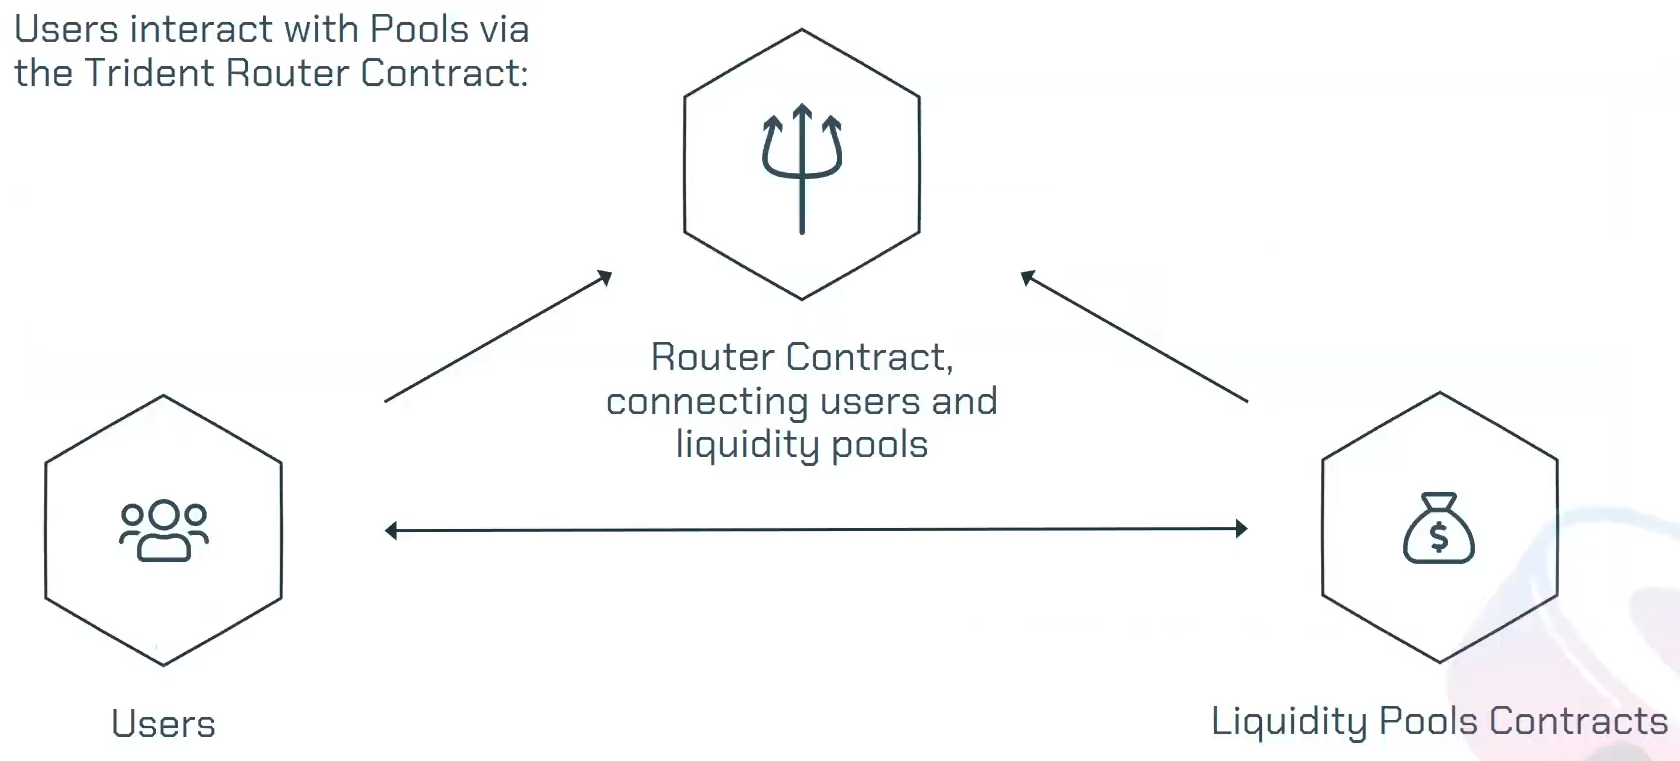
\includegraphics[width=\linewidth]{img/sushiswap_trident}
    \end{figure}

    In this scenario we have users, the router and the liquidity pools.
    All $3$ are manipulated in an interesting way.
    The property that we wish is the same that we have implemented earlier:

    $$
    \begin{pmatrix}
        \text{\texttt{totalLiquidity}},\\
        \text{\texttt{tokenA.balanceOf(system)}},\\
        \text{\texttt{tokenB.balanceOf(system)}}=\text{\texttt{0}}
    \end{pmatrix}\vee\begin{pmatrix}
        \text{\texttt{totalLiquidity}},\\
        \text{\texttt{tokenA.balanceOf(system)}},\\
        \text{\texttt{tokenB.balanceOf(system)}}\neq\text{\texttt{0}}
    \end{pmatrix}
    $$

    Earlier that we said that there is a correlation between the liquidation and the holding of the system.\\

    It's the same invariant we've seen earlier just written now specifically.
    It basically says that either total liquidity, token balance and token balance of the system are zero (all of them) or either all of them are nonzero.\\

    \pagebreak

    \begin{figure}[htbp!]
        \centering
        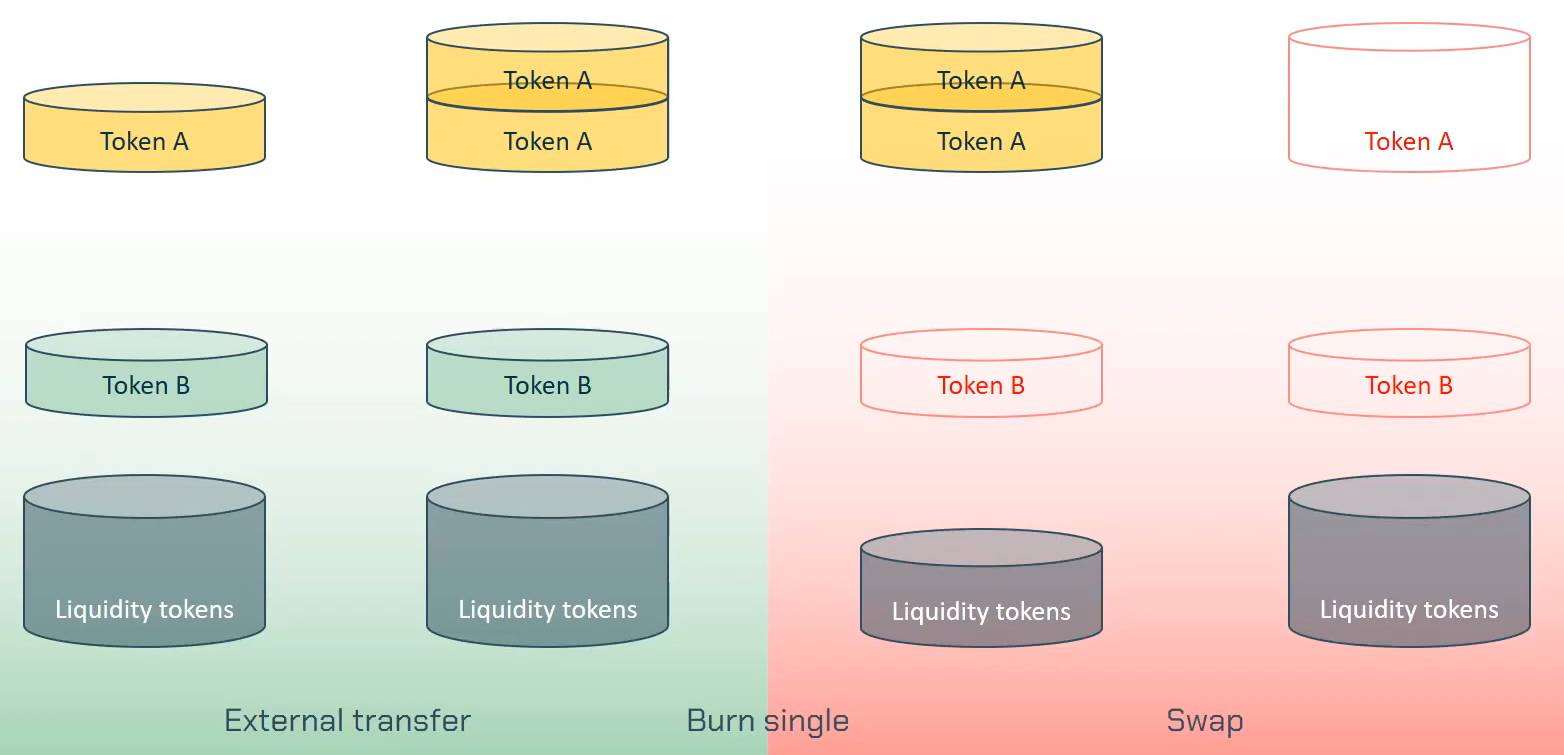
\includegraphics[width=\linewidth]{img/sushiswap_trident_bug}
    \end{figure}

    Basically you have token \texttt{A}, token \texttt{B} and a liquidity pool.
    Now you are doing external transfer: what happened is that you increase the amount of token \texttt{A}.
    However, there is this tricky scenario in which you increase the token in such a way that the internal data structure of the system is not aware of it.\\

    Say that now you are executing an operation called \texttt{Burn single}.
    What this operation does is to burn token \texttt{A} and, because the system is confused about the amount of token \texttt{A} you can burn, may leave you with one token or zero tokens.
    This is a case in which the invariant is broken.
    This looks bad already, but the question is: what can happen?\\


    So the liquidity tokens were reduced and, let's say, you were able to withdraw the token \texttt{B}.
    Now we are in this bad situation which allows you to swap this one token for everything, so you basically ended up replacing and taking all the money from the system.\\

    \pagebreak

    \section{A potential Spec of an ownable system}

    Now, tell me what's wrong about the following property:

    \begin{align*}
        &\text{\texttt{\{currentOwner}} = \text{\texttt{owner()}}\wedge\text{\texttt{other}}\neq\text{\texttt{currentOwner\}}}\\
        &\hspace{1cm}\text{\texttt{Op}}\\
        &\text{\texttt{\{owner()}}\neq\text{\texttt{currentOwner}}\vee\text{\texttt{owner}}\neq\text{\texttt{other\}}}\\
    \end{align*}

    What is wrong about this rule? Will it hold?\\

    This will always hold because the ``post" condition is vacuous.
    So, if you know that the \texttt{currentOwner} equals the \texttt{owner}, and \texttt{other} is not equal to \texttt{currentOwner}, then there is no way that this rule could be violated.\\

    When you run \texttt{Certora Prover}, it will tell you that rule holds, but this means nothing.
    So the Certora team is now incorporating into the tool the ability to check vacuous rules.\\

    The idea is that you want to check rules and the tool will inform you, in the case of the rules that hold, which of them are useful and which are not.

    \section{Suggested Software Life Cycle}

    How do people work with these methods?

    \begin{enumerate}
        \item\textbf{Design}: the best code starts with a good design backed by a whitepaper.
            Of course you can have bugs in this phase.
        \item\textbf{Spec, Code, Test}: from the design part on, you write the code and test.
            In addtion, it is also necessary to write the spec.
        \item\textbf{Testing}: then there is this manual procedure called QA or testing.
            Basically, either by hand or by means of certain tools, you run the code on some test input and you check if the spec is right or wrong.
            You can actually already identify some bugs in this phase, which is quite useful.
            Be it unit testing or system testing.\\

        \item\textbf{Spec Checking}: This is where \texttt{Certora} comes into play: they offer tools that check for vacuous tautology or spec violation.
            This reveals bugs in the spec.
        \item\textbf{Fuzzing}: tools like \texttt{Slither}.
            Think of it as a mechanism of generating more test input.
            It will basically augment your original test input with other test inputs that show you something about the spec.
        \item\textbf{Auditing}: manual step.
            It's a very very useful procedure where a human identifies other bugs in the design, spec, code\dots\\
            This step can be executed anytime, but since it's costly (because a human is involved) you will want to execute after doing all the automated steps.
        \item\textbf{Formal Verification}: by means of automated tools, formal verification will check the code and it can find bugs even after audition.\\

        If we have the right rules, we can identify bugs after the auditor, and even if we don't, it increases your knowledge of the code.\\

        The output of this procedure is a proof that the rules you rote are correct.
    \end{enumerate}

    At each of these phases, of course, you can go back.

    \section{Myths vs. Reality about Formal verification}

    \begin{table}[htbp!]
        \centering
        \begin{tabular}{|l|l|}
            \hline
            \textbf{Myths}&\textbf{Reality}\\
            \hline
            Formal Verification can & The biggest value of Formal \\
            only prove absence of bugs & Verification is finding bugs\\
            \hline
            Hardest problem is computational & Hardest problem is specification\\
            \hline
            Formal Verification is a one-time deal & Formal Verification guarantees \\
            & code upgrade safety\\
            \hline
        \end{tabular}
    \end{table}


    Although being a mature domain, Formal Verification still requires some thought.\\

    It is common to think that Formal Verification only produces proofs, but the biggest advantage is finding bugs in the rules.
    It is also of common wisdom that the hardest problem is computational, which is of course the case, but in many cases we can see that specification is equally hard and sometimes even a harder problem, because we are coming up with these essential rules of \texttt{DeFi}, like with liquidations.
    Also, it is a community effort.\\

    The last thing about Formal Verification, is the common thought of one-time deal, like proving the correctness of a compiler.
    In the case of \texttt{DeFi}, and many other evolving software, it's not a one-time deal.
    Every time you change the code you probably have to do auditing and Formal Verification, even if it's a tiny change in the code.\\

    This is where Formal Verification scales: you can run the rules again and again and again as part of the CR.\\

    There is no silver bullet for code correctness and Formal Verification is  required for code correctness.
    Formal Verification brings into the table the ability to the path: from ``Code is law" to ``Spec is law", and writing spec that people can read, critique and review.

\end{document}